\section{Results}
\label{sec:results}

We report the 16K slice unless stated. Positive relative reduction means the
specialized tokenizer uses fewer tokens. All values are reconciled against source
files by the claim registry (Appendix~\ref{app:verify}).

\paragraph{Primary result.} On the Azure cross-service holdout (five whole
held-out services, $n=964$ documents), the Azure tokenizer uses $240.18$ tokens
per $1{,}000$ UTF-8 bytes versus $379.30$ for the byte-matched General tokenizer,
a relative reduction of \reduc{36.68} (95\% paired-bootstrap CI
$[35.77\%, 37.62\%]$; document win rate $1.000$). Table~\ref{tab:main} and
Figure~\ref{fig:primary} summarize the result and its stability across
vocabulary sizes.

\begin{table}[t]
\centering
\caption{Main results at 16K: token reduction (\%) relative to the byte-matched
General tokenizer on the Azure cross-service holdout and on held-out general
English. Positive $=$ fewer tokens.}
\label{tab:main}
\small

\begin{tabular}{lrr}
\toprule
\textbf{Tokenizer (16K)} & \textbf{Azure cross-service} & \textbf{General English} \\
 & \textbf{reduction (\%)} & \textbf{reduction (\%)} \\
\midrule
Azure & $+36.68$ & $-34.75$ \\
Mixed (50/50) & $+34.21$ & $-4.39$ \\
General & $0$ (ref.) & $0$ (ref.) \\
\midrule
\multicolumn{3}{l}{\footnotesize Azure primary 95\% CI $[35.77, 37.62]$, win rate 1.0, $n=964$.} \\
\multicolumn{3}{l}{\footnotesize Positive $=$ specialized tokenizer uses fewer tokens per 1{,}000 UTF-8 bytes.} \\
\bottomrule
\end{tabular}

\end{table}

\begin{figure}[t]
\centering
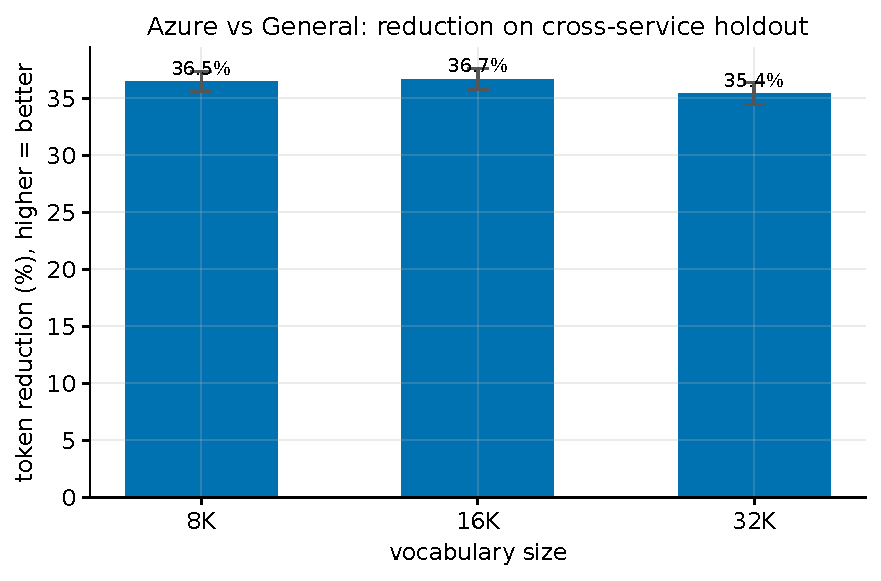
\includegraphics[width=0.62\linewidth]{fig01_primary.pdf}
\caption{Relative token reduction (\%) of the Azure vs byte-matched General
tokenizer on the Azure cross-service holdout, by vocabulary size, with 95\%
paired-bootstrap confidence intervals. Higher is better.}
\label{fig:primary}
\end{figure}

\paragraph{General-English regression (RQ2).} Full specialization has a cost: on
held-out general English the Azure tokenizer uses \reduc{34.75} more tokens than
General (95\% CI $[34.40\%, 35.10\%]$ more)---the direction reverses on
out-of-domain text.

\paragraph{Mixed-tokenizer tradeoff (RQ3).} The 50/50 Mixed tokenizer achieves a
\reduc{34.21} reduction on the Azure holdout---retaining \reduc{93.3} of the
Azure-only tokenizer's in-domain gain---while using only \reduc{4.39} more tokens
on held-out general English (Figure~\ref{fig:tradeoff}).

\begin{figure}[t]
\centering
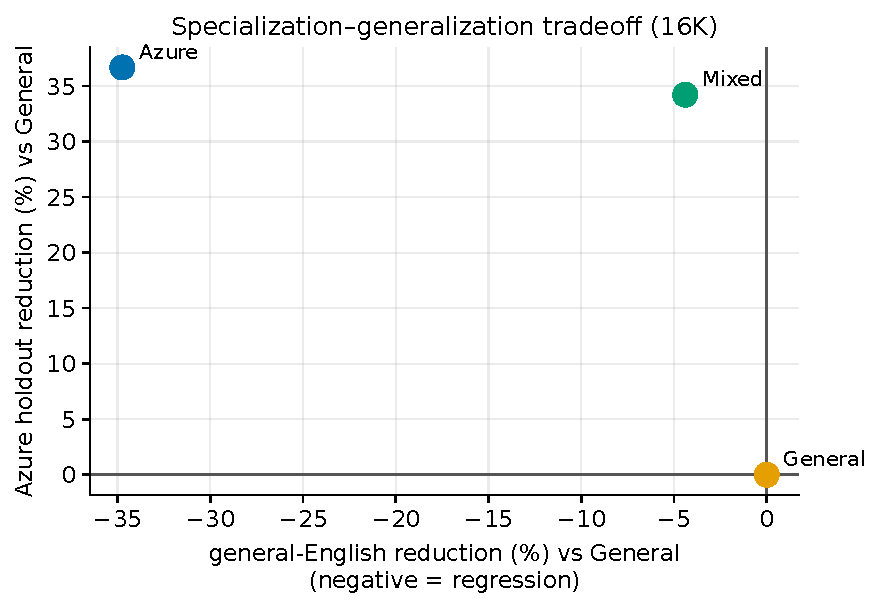
\includegraphics[width=0.6\linewidth]{fig02_tradeoff.pdf}
\caption{Specialization--generalization tradeoff at 16K: token reduction (\%)
relative to General on the Azure holdout (y) versus held-out general English (x).
Up and to the right is better on both axes.}
\label{fig:tradeoff}
\end{figure}

\paragraph{Transfer (RQ4).} The advantage decays with domain distance and persists
on non-Microsoft documentation: $+35.03\%$ (Azure same-service), $+32.94\%$
(Microsoft data), $+31.76\%$ (Microsoft DevOps), $+31.18\%$ (Kubernetes,
external), $+26.03\%$ (Microsoft architecture), and $+25.89\%$ (Microsoft
broad-enterprise); all confidence intervals exclude zero. Table~\ref{tab:transfer}
and Figure~\ref{fig:transfer} report transfer with the general-English regression.

\begin{table}[t]
\centering
\caption{Transfer of the Azure vs General reduction (\%, 16K) across evaluation
sets, plus vocabulary-size sensitivity on the principal holdout. Positive $=$
fewer tokens.}
\label{tab:transfer}
\small
\begin{tabular}{lr}
\toprule
\textbf{Evaluation set} & \textbf{Azure vs General reduction (\%)} \\
\midrule
Azure cross-service holdout (principal) & $+36.68$ \\
Azure same-service holdout & $+35.03$ \\
Microsoft data docs & $+32.94$ \\
Microsoft DevOps docs & $+31.76$ \\
Kubernetes (external technical) & $+31.18$ \\
Microsoft architecture docs & $+26.03$ \\
Microsoft broad-enterprise docs & $+25.89$ \\
General English & $-34.75$ \\
\midrule
\multicolumn{2}{l}{\footnotesize Vocabulary sensitivity (principal): 8K $+36.46$, 16K $+36.68$, 32K $+35.41$.} \\
\bottomrule
\end{tabular}

\end{table}

\begin{figure}[t]
\centering
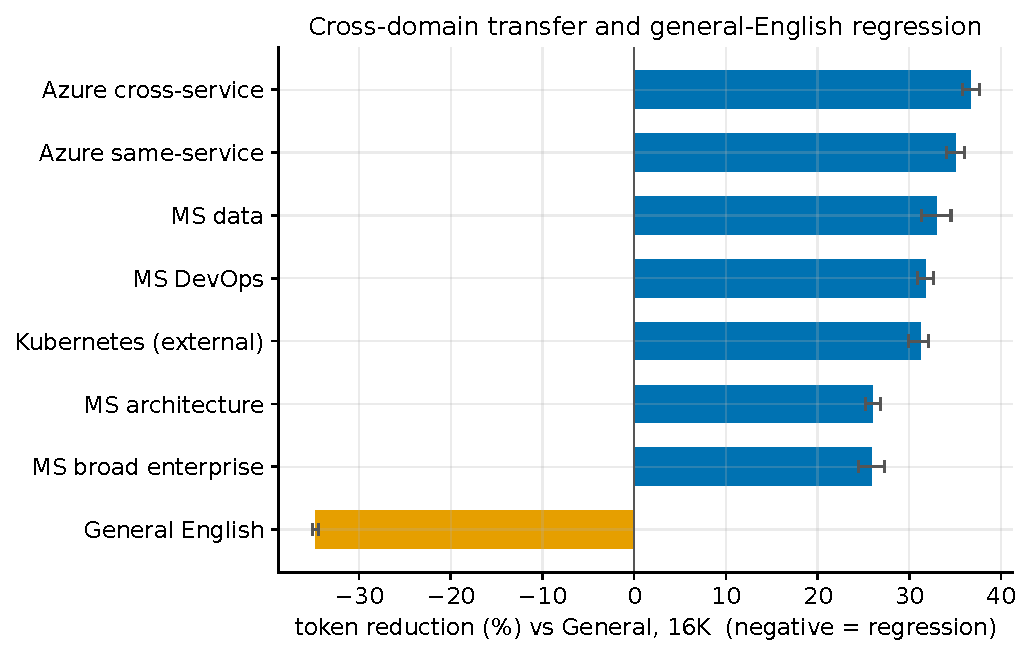
\includegraphics[width=0.72\linewidth]{fig03_transfer.pdf}
\caption{Azure vs General reduction (\%, 16K) across evaluation sets with 95\%
paired-bootstrap CIs. The general-English bar is negative (a regression).}
\label{fig:transfer}
\end{figure}

\paragraph{Vocabulary-size sensitivity (RQ5).} The reduction on the principal
holdout is stable across the tested range: \reduc{+36.46} (8K), \reduc{+36.68}
(16K), \reduc{+35.41} (32K) (Figure~\ref{fig:vocab}), suggesting corpus
composition mattered more than the tested vocabulary range.

\begin{figure}[t]
\centering
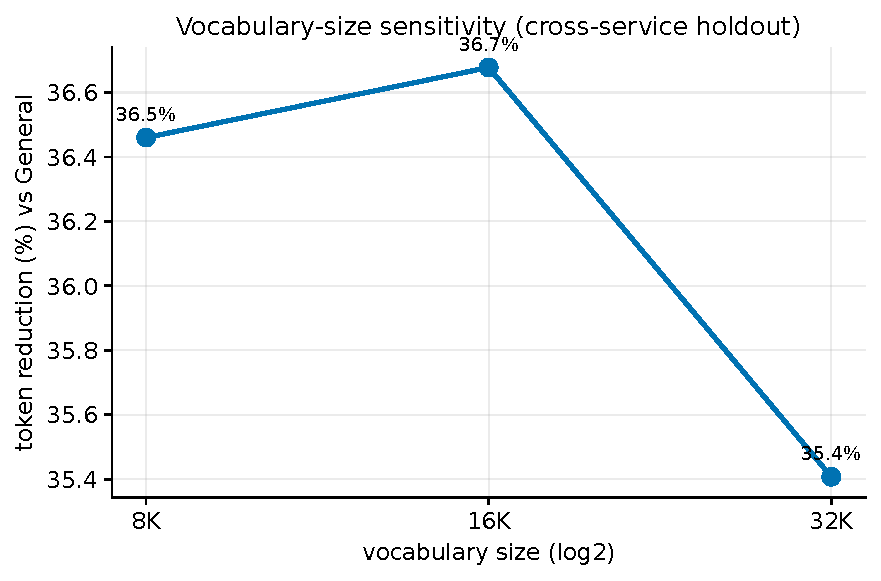
\includegraphics[width=0.58\linewidth]{fig04_vocab.pdf}
\caption{Vocabulary-size sensitivity: Azure vs General reduction (\%) on the
cross-service holdout at 8K/16K/32K.}
\label{fig:vocab}
\end{figure}

\paragraph{Content type (RQ6).} By dominant content type on the principal holdout:
prose-dominant documents ($n=900$) show \reduc{+36.75} (95\% CI
$[35.87\%, 37.63\%]$), headings \reduc{+37.49}, tables \reduc{+44.30}, and inline
code \reduc{+33.28} (Figure~\ref{fig:content}). Because the largest stratum
(prose) still shows a large reduction, the effect is not explained only by code
fences or configuration syntax.

\begin{figure}[t]
\centering
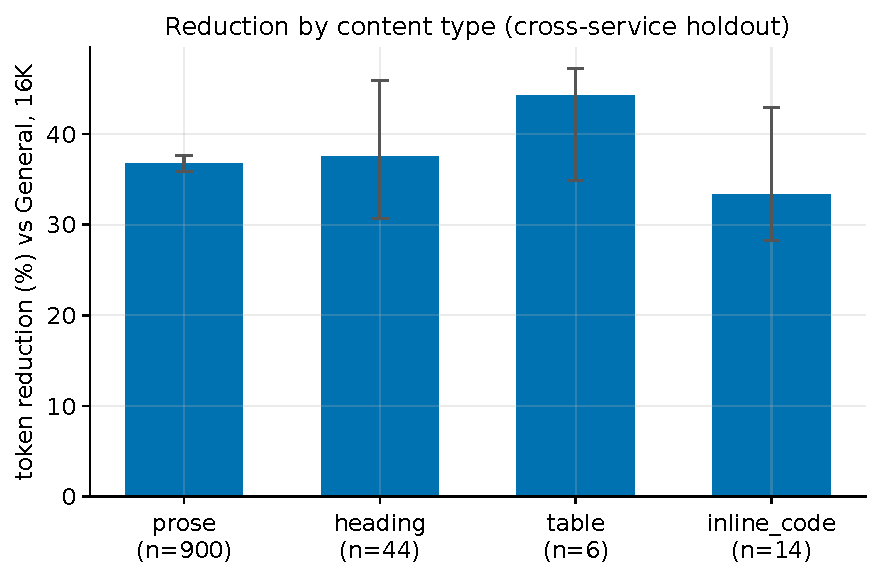
\includegraphics[width=0.58\linewidth]{fig05_content.pdf}
\caption{Reduction by dominant content type on the cross-service holdout (16K),
with 95\% CIs and per-stratum document counts.}
\label{fig:content}
\end{figure}

\paragraph{Coverage and runtime (RQ7).} Across $12$ encoders $\times$ $9$
evaluation sets ($59{,}160$ rows), reconstruction is exact ($100\%$ round-trip)
with zero unknown tokens. Median CPU tokenizer throughput is $5.1$--$5.5$\,MB/s
for the controlled tokenizers and $11.6$--$19.8$\,MB/s for the \texttt{tiktoken}
baselines (Figure~\ref{fig:runtime}); the controlled tokenizers compress more but
run slower on CPU than the production-optimized baselines. Compression and CPU
throughput are distinct dimensions, and CPU throughput is not model-serving
throughput. Table~\ref{tab:runtime} summarizes coverage and runtime.

\begin{table}[t]
\centering
\caption{Coverage and CPU-runtime summary. CPU tokenizer throughput is not
model-serving throughput.}
\label{tab:runtime}
\small

\begin{tabular}{lr}
\toprule
\textbf{Measure} & \textbf{Value} \\
\midrule
Evaluation rows & 59,160 (12 encoders $\times$ 9 sets) \\
Exact round-trip & 100\% \\
Unknown tokens (\texttt{[UNK]}) & 0 \\
CPU throughput, Track A (MB/s) & 5.13--5.47 \\
CPU throughput, Track B \texttt{tiktoken} (MB/s) & 11.61--19.83\\
Automated verification gate & 8/8 \\
\bottomrule
\end{tabular}

\end{table}

\begin{figure}[t]
\centering
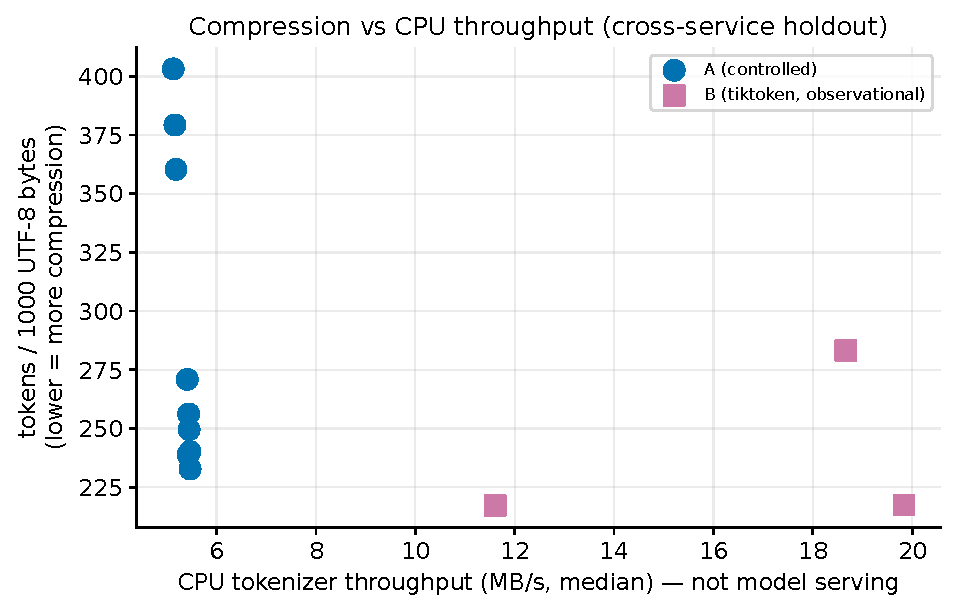
\includegraphics[width=0.62\linewidth]{fig06_runtime.pdf}
\caption{Compression (tokens per $1{,}000$ UTF-8 bytes, lower is better) versus
measured CPU tokenizer throughput on the cross-service holdout. Track A are the
controlled tokenizers; Track B (\texttt{tiktoken}) are observational baselines.}
\label{fig:runtime}
\end{figure}
